图\ref{fig:1}中的脉冲$g_2(t)$的脉冲宽度是多少?占空比是多少?

\begin{myfigure}
    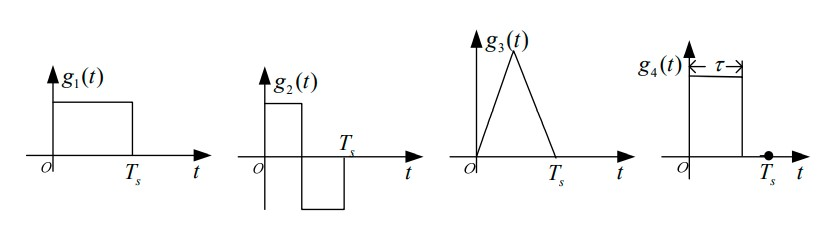
\includegraphics[scale=0.65]{image/1.jpg}
    \caption{几种不同的基带脉冲波形. 它们具有相同的能量, 其中$g_4(t)$的占空比小于1, 前3种是全占空的.}
    \label{fig:1}
\end{myfigure}

\begin{solution}
    % 这里写你的答案
\end{solution}
